\documentclass[10pt,t]{beamer}
\usetheme{Heverlee}





\usepackage{times}

\usepackage{amsmath,amssymb}
\usepackage[latin1]{inputenc}

\usepackage{array}
\usepackage{amsmath}
\usepackage{amsthm}
\usepackage{amssymb}
\usepackage{graphicx}
\usepackage{hyperref}
\usepackage{longtable}
\usepackage{pdfpages}
\usepackage{eurosym} 
\usepackage{xcolor}

\usepackage[absolute,overlay]{textpos}
\usepackage{everypage}

\usepackage{pgf}
\usepackage{tikz}


\usepackage{setspace}  
\usepackage{colortbl}
\usepackage{graphicx}

\DeclareGraphicsExtensions{.jpg,.pdf,.mps,.png}



%%% QUICK OPTIONS:
% (A) Math font without serifs, enable line below to make math serif:
    %\usefonttheme[onlymath]{serif}

% (B) Re-define primary colour by adjusting the RGB values
    %\definecolor{pblue}	{RGB}{206,125,66}

% (C) Title page graphic (optional) --- this is not for the background image, see \usebackgroundtemplate to change that ---
    %\titlegraphic{\includegraphics[height=2.7cm]{example_figure.pdf}}

% (D) Add logo to bottom right-corner (optional)
    \logo{
\includegraphics[height=0.7cm]{logo.png}\hspace{12pt}\vspace{-6pt}}      

% (E) Choose one (or none) of these lines to add footline bar on all frames
    %\setbeamertemplate{footline}[infoline]  % author, title, insitute
    %\setbeamertemplate{footline}[navigation] % dots swhowing progress
    %\setbeamertemplate{footline}[navsym] % navigation symbols

% (F) Widescreen 16:9 ratio
    %\usepackage[orientation=landscape,size=custom,width=16,height=9,scale=0.45,debug]{beamerposter} 



%%% TITLE PAGE INFO:
\title[Heverlee \LaTeX\ Beamer theme]{Heverlee Beamer theme}
\subtitle{\textbackslash usetheme\{Heverlee\}}
\author{John Doe}
\institute{Placeholder University}
\date{September 2020}

% Text inside {} is used on the title page. Text inside [] is optional, and is used in footline bar (if [] is omitted then text from {} will be used in both ; if [] is specified but left empty then the footline will not show any text)




 %%
 %%  0. TITLE PAGE and TABLE OF CONTENT
 %%
\begin{document}
% Title page

{
% Change image, or delete this line to remove background image
\usebackgroundtemplate{ \parbox[b][\paperheight][b]{\paperwidth}{\centering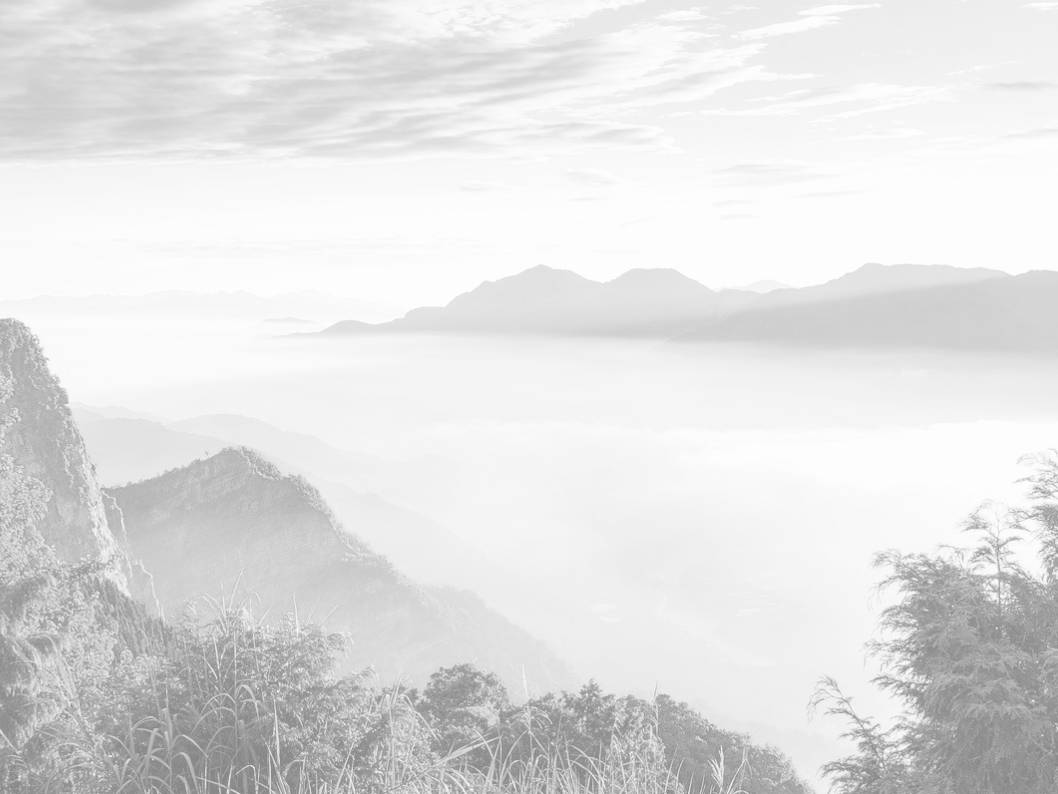
\includegraphics[width=\paperwidth]{Background/bg_alishan.jpg}}} 
 %   abudhabi      cherry      forest      river
 %   alishan       chobe       leuven      sanfancisco
 %   blueprint     columns     library     uyuni
 %   bokeh         flowers     newyork     winter

%\setbeamercolor{background canvas}{bg=lgray}  % make background light gray

\begin{frame}[plain,noframenumbering]
    \titlepage
\end{frame}
}		


% Table of contents slide
\begin{frame}{Outline}
	\vskip 2mm
	\hfill	{\large \parbox{.95\textwidth}{\tableofcontents[hideothersubsections]}}
\end{frame}

\section{Rambling Section}

\subsection{First Subsection}
	
\begin{frame}
	Here is some rambling text
	\begin{enumerate}
		\item List item 1
		\item List item 2
	\end{enumerate}
\end{frame}

\begin{frame}{First order linear difference equation}

	\transwipe
	
	\begin{textblock*}{12cm}(0.5cm,1cm)
	
	\begin{block}{General expression (constant coefficients)}
	For $\alert{\alpha}, \textcolor{blue}{\beta} \in \mathbb{C}$, $\quad n\geqslant 0$,
	\begin{equation*}
	x_{n+1} = \alert{\alpha} \, x_n + \textcolor{blue}{\beta}.
	\end{equation*}
	Eventually, $x_0$ is given as the initial term.
	\end{block}
	
	\end{textblock*}
	
	\pause
	
	\vspace{3cm}
	
	\alert{Unknown}: The sequence $\{x_n\}_{n\geqslant0}$ of complex numbers.
	
	\vspace{1cm}
	
	\alert{Objective}: To find the unknown $\{x_n\}_{n\geqslant0}$ (if it exists).
	
	
	\vspace{1cm}
	
	\alert{Particular case}. If $\alert{\alpha} =0$, the solution is the constant sequence $\{x_n\}_{n\geqslant0} = \{\beta\}_{n\geqslant0}.$
	
	
	\end{frame}
	
	%%%%%%%%%%%%%%%%%%%%%%%%%%%%%%%%%%%%%%%%%%%%%%%%%%%%%%%%%5
	
	\begin{frame}{First order linear difference equation}
	
	\transwipe
	
	\begin{textblock*}{12cm}(0.5cm,1cm)
	
	\begin{block}{General expression (constant coefficients)}
	For $\alert{\alpha}, \textcolor{blue}{\beta} \in \mathbb{C}$, $\quad n\geqslant 0$,
	\begin{equation*}
	x_{n+1} = \alert{\alpha} \, x_n + \textcolor{blue}{\beta}.
	\end{equation*}
	Eventually, $x_0$ is given as the initial term.
	\end{block}
	
	\end{textblock*}
	
	\vspace{3cm}
	
	Particular case:  \textcolor{red}{Arithmetic progression}.  For $\alert{\alpha} = 1$,
	$$
	x_{n+1} = x_n + \textcolor{blue}{\beta}, \quad n\geqslant 0.
	$$
	
	\vspace{1cm}
	
	Solution: \quad $x_{n} = x_0 + n\,\textcolor{blue}{\beta}, \quad n\geqslant 0.$
	 
	\end{frame}
	
	%%%%%%%%%%%%%%%%%%%%%%%%%%%%%%%%%%%%%%%%%%%%%%%%%%%%%%%%%5
	
	\begin{frame}{First order linear difference equation}
	
	\transwipe
	
	\begin{textblock*}{12cm}(0.5cm,1cm)
	
	\begin{block}{General expression (constant coefficients)}
	For $\alert{\alpha}, \textcolor{blue}{\beta} \in \mathbb{C}$, $\quad n\geqslant 0$,
	\begin{equation*}
	x_{n+1} = \alert{\alpha} \, x_n + \textcolor{blue}{\beta}.
	\end{equation*}
	Eventually, $x_0$ is given as the initial term.
	\end{block}
	
	\end{textblock*}
	
	\vspace{3cm}
	
	
	Particular case: \textcolor{red}{Geometric progression}.  For $\textcolor{blue}{\beta} = 0$, 
	$$
	x_{n+1} = \alert{\alpha}\, x_n, \quad n\geqslant 0.
	$$
	
	\vspace{1cm}
	
	Solution: \quad $x_{n} = x_0 \, \alert{\alpha}^n, \quad n\geqslant 0.$
	
	
	\end{frame}
	
	%%%%%%%%%%%%%%%%%%%%%%%%%%%%%%%%%%%%%%%%%%%%%%%%%%%%%%%%%%%%%%%%%%%%%%%%%%%%%%%%
	
	\begin{frame}{Solving the first order linear difference equation}
	
	\transwipe
	
	\begin{textblock*}{12cm}(0.5cm,1cm)
	
	\begin{block}{Proposition 1} Let $\alert{\alpha}, \textcolor{blue}{\beta} \in \mathbb{C}$, and $\alert{\alpha} \neq 1$. Then, the difference equation
	\begin{equation}\label{eq-lin}
	x_{n+1} = \alert{\alpha} \,x_n + \textcolor{blue}{\beta}, \quad n\geqslant 0,
	\end{equation}
	has a unique constant solution in the form $\displaystyle{x_{*} = \frac{\textcolor{blue}{\beta}}{1-\alert{\alpha}}}$
	\end{block}
	
	\end{textblock*}
	
	\vspace{4cm}
	
	The value $x_*$ is usually called \textcolor{red}{equilibrium}.
	
	\vspace{1cm}
	
	\textcolor{blue}{Proof.} A constant solution satisfies $x_n = x_*$, $n\geqslant0$. Substituting in \eqref{eq-lin}, we get
	$$
	x_{*} = \alert{\alpha} \,x_* + \textcolor{blue}{\beta}.
	$$
	Grouping terms, we get the announced expression.
	\end{frame}
	
	
	%%%%%%%%%%%%%%%%%%%%%%%%%%%%%%%%%%%%%%%%%%%%%%%%%%%%%%%%%%%%%%%%%%%%%%%%%%%%%%%%

\end{document}